\documentclass[10pt,reqno]{amsart}

\usepackage[T1]{fontenc}
\usepackage{newtxtext,newtxmath}
\let\Bbbk\relax
\usepackage{amsmath,amssymb}
\usepackage{microtype}
\usepackage[margin=0.98in]{geometry}
\usepackage{tikz}
\usetikzlibrary{arrows.meta}
\usepackage[numbers]{natbib}
\usepackage[colorlinks=true,linkcolor=blue!65!black,citecolor=blue!65!black,urlcolor=blue!65!black]{hyperref}

\begin{document}
\title{Thermodynamic compatibility and the emergence of chemical organization}
\maketitle

\section{Physical reaction space}

A chemical network has a fixed set of elementary reactions, but its
present composition determines which of them can occur. We divide the
species counts into an internal state $x$ and an environment $z$, with
$n=(x,z)\in\mathbb N_0^N$. Reaction $r$ changes $n$ by a stoichiometric
vector $\nu_r$. Collecting these vectors gives
\begin{equation}
\mathbf S=\begin{bmatrix}\mathbf S_x\\\mathbf S_z\end{bmatrix}
=\begin{bmatrix}\nu_1&\cdots&\nu_M\end{bmatrix}=\mathbf Z\mathbf B,
\label{eq:stoichiometry}
\end{equation}
where $\mathbf B$ is the incidence matrix of the graph of chemical
complexes and $\mathbf Z$ gives the species composition of each complex
\cite{vanderschaft2013balanced}. With physical propensities $w_r(n)$,
the stochastic generator is
\begin{equation}
(\mathsf L\varphi)(n)=\sum_r w_r(n)
\bigl[\varphi(n+\nu_r)-\varphi(n)\bigr].
\label{eq:generator}
\end{equation}
Reactant availability and catalysis enter through $w_r(n)$; their
products therefore change subsequent reaction propensities without an
independent adaptation law \cite{gillespie1977}. The environment is the
source of chemical resources, not an external repair mechanism for $x$.

\section{Thermodynamic compatibility}

Fix the chemical potentials $\mu_z$ of the maintained environmental
reservoirs, and let $\mu_x$ denote internal chemical potentials. For
any selected collection of reactions, orient each column of
$\mathbf S$ along the direction required for its operation. Their
affinities are
\begin{equation}
 a=-\mathbf S_x^\top\mu_x-\mathbf S_z^\top\mu_z.
\label{eq:affinities}
\end{equation}
Strictly positive $a_r$ permits positive net flux in the selected
direction for a thermodynamically consistent elementary reaction.
A nonnegative internal turnover flux $q\ne0$ obeys
$\mathbf S_xq=0$. Its total chemical driving is
\begin{equation}
q^\top a=-\mu_z^\top\mathbf S_zq.
\label{eq:cycle-work}
\end{equation}
Thus a collection of required directions is impossible if it contains
such a $q$ with nonpositive environmental work. This is the
thermodynamic cycle obstruction, not a test for autocatalysis itself
\cite{rao2016crn}.

The restriction can be expressed through the maximum common affinity
margin. If the normalized cycle set
$\{q\geq0:\mathbf S_xq=0,\ \mathbf1^\top q=1\}$ is nonempty, linear
programming duality yields
\begin{equation}
\delta_*:=\max_{\mu_x}\min_r a_r
=\min_{\substack{q\geq0,\ \mathbf S_xq=0\\\mathbf1^\top q=1}}
\bigl(-\mu_z^\top\mathbf S_zq\bigr).
\label{eq:margin}
\end{equation}
Here internal potentials are allowed to vary without bounds. Positive
$\delta_*$ is equivalent to simultaneous strict directional feasibility
under this assumption. The margin is measured in energy per reaction
event and does not determine reaction rates, stability, or persistence.
If the normalized cycle set is empty, the margin is unbounded above in
this unconstrained problem. Finite concentrations, conserved totals,
and kinetic restrictions can narrow the feasible region.

\section{Two competing autocatalytic cores}

Kosc and collaborators identified two autocatalytic cores that share
reactions and admit compatible stoichiometric production fluxes, yet
cannot operate simultaneously with thermodynamically consistent
mass-action kinetics \cite{blokhuis2020,kosc2025}. Their six reaction directions are
\begin{equation}
\begin{aligned}
R_1:&\ X_1\to B+X_2, &R'_1:&\ X'_1\to A+X'_2,\\
R_2:&\ X_2+X'_2\to X_3, &R_3:&\ X_3\to2X_4,\\
R_4:&\ A+X_4\to X_1, &R'_4:&\ B+X_4\to X'_1.
\end{aligned}
\label{eq:cores}
\end{equation}
The cores are $(R_1,R_2,R_3,R_4)$ and
$(R'_1,R_2,R_3,R'_4)$. One occurrence of every reaction gives zero
net change in every species, so $\mathbf Sq=0$ for
$q=(1,1,1,1,1,1)^\top$. Equation~\eqref{eq:cycle-work} forces
$\sum_r a_r=0$: their six prescribed directions cannot all have
positive affinity. This recovers the published incompatibility.
Equivalently, with
$\theta=\mu_B+\mu_{X_2}-\mu_A-\mu_{X_4}$, the first core
requires $\theta<0$ whereas the second requires $\theta>0$.

As a separate, illustrative extension, couple $R_1$ to conversion of
an environmental fuel $F$ into waste $W$,
$X_1+F\to B+X_2+W$. The internal stoichiometry remains unchanged,
while the full cycle now consumes one fuel molecule. If
$\Delta\mu=\mu_F-\mu_W$, its affinity sum is $\Delta\mu$.
The first core now requires $\theta<\Delta\mu$, allowing its
necessary potential window to overlap with that of the second core.
The normalized nonnegative kernel of $\mathbf S_x$ is the single
vector $\mathbf1/6$, giving the exact margin
\begin{equation}
\delta_*={\Delta\mu}/{6}.
\label{eq:fuel-margin}
\end{equation}
The two cores and the chemical-potential window for their joint
operation are shown in Fig.~\ref{fig:compatibility}. The latter
compares necessary inequalities; the affinity margin provides the
stronger simultaneous-direction criterion.

\begin{figure}[htb!]
\centering
\begin{minipage}[c]{0.48\linewidth}
\centering
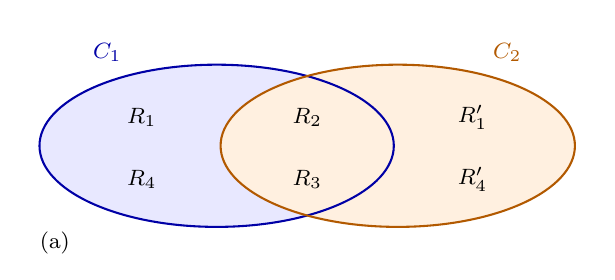
\begin{tikzpicture}[font=\footnotesize]
\path[use as bounding box] (-3.55,-1.35) rectangle (3.55,1.50);
\fill[blue!9] (-1.15,0) ellipse (2.25cm and 1.03cm);
\fill[orange!12] (1.15,0) ellipse (2.25cm and 1.03cm);
\draw[blue!65!black,line width=0.75pt] (-1.15,0) ellipse (2.25cm and 1.03cm);
\draw[orange!70!black,line width=0.75pt] (1.15,0) ellipse (2.25cm and 1.03cm);
\node[blue!65!black] at (-2.54,1.18) {$C_1$};
\node[orange!70!black] at (2.54,1.18) {$C_2$};
\node at (-2.10,0.36) {$R_1$};
\node at (-2.10,-0.43) {$R_4$};
\node at (0,0.36) {$R_2$};
\node at (0,-0.43) {$R_3$};
\node at (2.10,0.36) {$R'_1$};
\node at (2.10,-0.43) {$R'_4$};
\node[anchor=west] at (-3.52,-1.23) {(a)};
\end{tikzpicture}
\end{minipage}\hfill
\begin{minipage}[c]{0.48\linewidth}
\centering
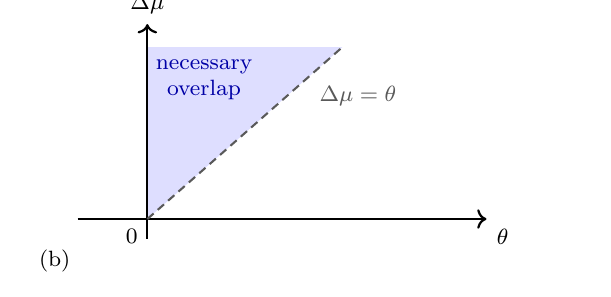
\begin{tikzpicture}[font=\footnotesize,x=1cm,y=1cm]
\path[use as bounding box] (-0.45,-0.66) rectangle (6.6,2.40);
\begin{scope}[shift={(1.07,-0.03)},x=1.18cm,y=1.04cm]
\fill[blue!13] (0,0) -- (0,2.1) -- (2.1,2.1) -- cycle;
\draw[->,line width=0.8pt] (-0.75,0) -- (3.65,0)
node[below right] {$\theta$};
\draw[->,line width=0.8pt] (0,-0.24) -- (0,2.38)
node[above] {$\Delta\mu$};
\draw[densely dashed,black!65,line width=0.75pt] (0,0) -- (2.1,2.1)
node[pos=0.83,below right] {$\Delta\mu=\theta$};
\node[blue!65!black,align=center] at (0.61,1.70)
{necessary\\overlap};
\node[below left] at (0,0) {$0$};
\end{scope}
\node[anchor=west] at (-0.43,-0.56) {(b)};
\end{tikzpicture}
\end{minipage}
\caption{Reaction-core overlap and thermodynamic compatibility.
(a) The cores share reactions $R_2,R_3$; this is a reaction-set
schematic, not the complex graph. (b) Fuel driving opens the necessary
window $0<\theta<\Delta\mu$ (blue) for the two sets of forward
reactions. A positive margin $\delta_*$ is the full directional
feasibility test under unrestricted internal potentials.}
\label{fig:compatibility}
\end{figure}

Fuel driving can therefore remove the obstruction to simultaneous
\emph{reaction directions}. It does not establish a kinetically
maintained state or simultaneous autocatalytic growth.

\section{Stochastic baseline and limitation}

The six-reaction example contains a conservation law that restricts
its possible dynamics. With $A,B,F,W$ buffered and the other six
species internal, the positive vector
$\ell=(1,1,2,1,1,1)^\top$ obeys
$\ell^\top\mathbf S_x=0$, so the internal pool
$m=\ell^\top x$ is fixed. Moreover,
$\ker\mathbf S_x=\operatorname{span}\{\mathbf1\}$.
Thus any stationary reaction currents must satisfy
\begin{equation}
\langle v_1\rangle=\langle v'_1\rangle
=\langle v_2\rangle=\langle v_3\rangle
=\langle v_4\rangle=\langle v'_4\rangle=J.
\label{eq:one-current}
\end{equation}
There are no independent stationary currents associated with the two
cores. The state $x=0$ is also absorbing: the original reactions
cannot assemble an internal organization from an empty system.

For a dynamical check, we solved the finite-state chemical master
equation with reversible mass-action rates, buffered
$A=B=W=1$, $F=\exp(\beta\Delta\mu)$, unit bare rate
constants, and dimensionless volume $4$. For $m=4,6,8$,
fuel driving first raises $J$ but subsequently suppresses it
through depletion of $X'_2$, which is required by the shared
reaction $X_2+X'_2\rightleftharpoons X_3$.
This negative differential response is a known chemical phenomenon
\cite{falasco2019}; the calculation is a baseline, not a novel
selection mechanism. The exact stationary solver and plotting script
are in \texttt{experiments/cores.py}.

Thermodynamic feasibility can therefore be separated from
actual throughput, but this model alone cannot demonstrate spontaneous
selection among independently maintained organizations. Studying that
phenomenon requires physical precursor-to-component synthesis and
turnover that break the conserved internal pool, with rates derived
from the expanded reaction network rather than a prescribed adaptive
feedback \cite{peng2022hierarchy}.

\bibliographystyle{unsrtnat}
\begingroup\footnotesize\bibliography{refs}\endgroup
\end{document}
